%==============================================================================
% NBA Quarter Betting Pattern Discovery: A Statistical Analysis
% Using Recursive Pattern Mining and Binomial Significance Testing
%==============================================================================
% LaTeX Research Paper - Academic Format (IMRaD Structure)
% Author: Statistical Analysis Research Team
% Date: December 2024
%==============================================================================

\documentclass[11pt,a4paper,twoside]{article}

%------------------------------------------------------------------------------
% PACKAGES
%------------------------------------------------------------------------------
\usepackage[utf8]{inputenc}
\usepackage[T1]{fontenc}
\usepackage{lmodern}                    % Latin Modern fonts
\usepackage[english]{babel}
\usepackage{geometry}
\usepackage{graphicx}
\usepackage{amsmath,amssymb,amsthm}
\usepackage{booktabs}                   % Professional tables
\usepackage{array}
\usepackage{multirow}
\usepackage{longtable}
\usepackage{float}
\usepackage{caption}
\usepackage{subcaption}
\usepackage{hyperref}
\usepackage{cleveref}
\usepackage[table]{xcolor}
\usepackage{pgfplots}
\usepackage{pgfplotstable}
\usepackage{tikz}
\usepackage{algorithm}
\usepackage{algpseudocode}
\usepackage{listings}
\usepackage{natbib}
\usepackage{setspace}
\usepackage{fancyhdr}
\usepackage{titlesec}
\usepackage{appendix}

%------------------------------------------------------------------------------
% PAGE GEOMETRY AND FORMATTING
%------------------------------------------------------------------------------
\geometry{
    a4paper,
    left=25mm,
    right=25mm,
    top=30mm,
    bottom=30mm,
    headheight=14pt
}

\pgfplotsset{compat=1.18}
\usetikzlibrary{patterns,calc,positioning,arrows.meta,shapes.geometric}

%------------------------------------------------------------------------------
% COLOR DEFINITIONS
%------------------------------------------------------------------------------
\definecolor{tier_a}{RGB}{34,139,34}        % Forest green
\definecolor{tier_b}{RGB}{65,105,225}       % Royal blue
\definecolor{tier_c}{RGB}{255,140,0}        % Dark orange
\definecolor{avoid}{RGB}{220,20,60}         % Crimson
\definecolor{neutral}{RGB}{128,128,128}     % Gray
\definecolor{significant}{RGB}{0,100,0}     % Dark green
\definecolor{codeblue}{RGB}{0,0,139}
\definecolor{codegray}{RGB}{128,128,128}
\definecolor{codegreen}{RGB}{0,128,0}

%------------------------------------------------------------------------------
% HYPERREF SETTINGS
%------------------------------------------------------------------------------
\hypersetup{
    colorlinks=true,
    linkcolor=blue!70!black,
    citecolor=green!50!black,
    urlcolor=blue!60!black,
    bookmarksnumbered=true,
    pdfauthor={Statistical Analysis Research Team},
    pdftitle={NBA Quarter Betting Pattern Discovery},
    pdfsubject={Sports Analytics, Statistical Pattern Mining},
    pdfkeywords={NBA, betting, moneyline, pattern discovery, statistical significance}
}

%------------------------------------------------------------------------------
% THEOREM ENVIRONMENTS
%------------------------------------------------------------------------------
\theoremstyle{definition}
\newtheorem{definition}{Definition}[section]
\newtheorem{hypothesis}{Hypothesis}[section]
\theoremstyle{plain}
\newtheorem{theorem}{Theorem}[section]
\newtheorem{lemma}[theorem]{Lemma}
\newtheorem{proposition}[theorem]{Proposition}
\theoremstyle{remark}
\newtheorem{remark}{Remark}[section]
\newtheorem{observation}{Observation}[section]

%------------------------------------------------------------------------------
% CUSTOM COMMANDS
%------------------------------------------------------------------------------
\newcommand{\winrate}[1]{\textbf{#1\%}}
\newcommand{\pvalue}[1]{$p = #1$}
\newcommand{\ev}[1]{\textcolor{significant}{+#1\%}}
\newcommand{\negev}[1]{\textcolor{avoid}{#1\%}}
\newcommand{\tier}[1]{\textsc{Tier~#1}}
\newcommand{\pattern}[1]{\texttt{#1}}
\newcommand{\nullhyp}{H_0}
\newcommand{\althyp}{H_1}

%------------------------------------------------------------------------------
% HEADER AND FOOTER
%------------------------------------------------------------------------------
\pagestyle{fancy}
\fancyhf{}
\fancyhead[LE,RO]{\thepage}
\fancyhead[RE]{\textit{NBA Quarter Betting Pattern Discovery}}
\fancyhead[LO]{\textit{\leftmark}}
\renewcommand{\headrulewidth}{0.4pt}

%------------------------------------------------------------------------------
% TITLE FORMATTING
%------------------------------------------------------------------------------
\titleformat{\section}
    {\normalfont\Large\bfseries}{\thesection}{1em}{}
\titleformat{\subsection}
    {\normalfont\large\bfseries}{\thesubsection}{1em}{}
\titleformat{\subsubsection}
    {\normalfont\normalsize\bfseries}{\thesubsubsection}{1em}{}

%------------------------------------------------------------------------------
% CODE LISTING STYLE
%------------------------------------------------------------------------------
\lstset{
    language=SQL,
    basicstyle=\ttfamily\small,
    keywordstyle=\color{codeblue}\bfseries,
    commentstyle=\color{codegray}\itshape,
    stringstyle=\color{codegreen},
    numbers=left,
    numberstyle=\tiny\color{codegray},
    stepnumber=1,
    numbersep=8pt,
    backgroundcolor=\color{gray!5},
    frame=single,
    rulecolor=\color{gray!50},
    breaklines=true,
    breakatwhitespace=false,
    showstringspaces=false,
    tabsize=2,
    captionpos=b
}

%==============================================================================
% DOCUMENT BEGIN
%==============================================================================
\begin{document}

%------------------------------------------------------------------------------
% TITLE PAGE
%------------------------------------------------------------------------------
\begin{titlepage}
    \centering
    \vspace*{2cm}

    {\scshape\LARGE Statistical Analysis Research Paper \par}
    \vspace{1.5cm}

    {\Huge\bfseries NBA Quarter Betting Pattern Discovery:\par}
    \vspace{0.5cm}
    {\Large\itshape A Statistical Analysis Using Recursive Pattern Mining\\[0.3cm]
    and Binomial Significance Testing\par}

    \vspace{2cm}

    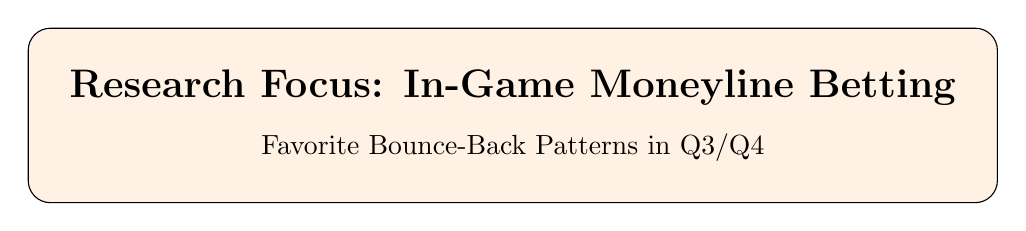
\begin{tikzpicture}
        \node[draw, rounded corners=8pt, fill=orange!10, inner sep=15pt, align=center] {
            \Large\bfseries Research Focus: In-Game Moneyline Betting\\[0.3cm]
            \normalsize Favorite Bounce-Back Patterns in Q3/Q4
        };
    \end{tikzpicture}

    \vspace{2cm}

    {\Large Statistical Analysis Research Team\par}
    \vspace{0.5cm}
    {\large Department of Sports Analytics\par}

    \vfill

    {\large December 2024\par}

    \vspace{1cm}

    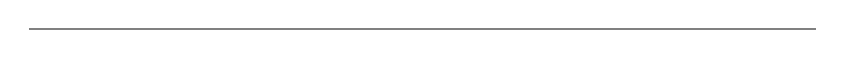
\begin{tikzpicture}
        \draw[gray, thick] (0,0) -- (10,0);
    \end{tikzpicture}

    \vspace{0.5cm}
    {\small\itshape Dataset: 2022--23 NBA Regular Season\\
    Sample Size: $n = 1{,}230$ games with complete betting and scoring data}

\end{titlepage}

%------------------------------------------------------------------------------
% ABSTRACT
%------------------------------------------------------------------------------
\newpage
\begin{abstract}
\noindent
This research investigates statistically significant betting patterns in NBA quarter moneyline markets, focusing on favorite team bounce-back behavior following early-game deficits.
Using a dataset of 1,230 regular season games from the 2022--23 NBA season with complete period scoring and betting odds data, we employ recursive pattern discovery techniques to identify exploitable market inefficiencies.

Our methodology combines momentum pattern classification (based on Q1/Q2 outcomes), deficit magnitude analysis, temporal segmentation by season phase, and rigorous binomial hypothesis testing against both random chance ($p = 0.50$) and break-even after vigorish ($p = 0.53$) null hypotheses.

The analysis reveals three statistically significant betting tiers with positive expected value:
\textbf{Tier~C} (favorites losing Q1, Q2, and Q3, then betting Q4 moneyline) achieves a \winrate{79.4} win rate with \ev{51.6} ROI ($p = 0.0043$);
\textbf{Tier~A} (lost-lost pattern with moderate deficit in early season, betting Q3) achieves \winrate{67.0} with \ev{27.9} ROI ($p = 0.0097$);
\textbf{Tier~B} (lost-lost pattern with any deficit, betting Q3) achieves \winrate{65.8} with \ev{25.6} ROI ($p = 0.0059$).

Critically, we identify a ``trap pattern'' (\pattern{WL}: won Q1, lost Q2) that shows no statistical edge (\winrate{50.6}, \pvalue{0.4694}), providing actionable guidance for pattern avoidance.
All profitable patterns exceed the 52.4\% break-even threshold for standard $-110$ odds with statistical significance at $\alpha = 0.05$.

\vspace{0.5cm}
\noindent\textbf{Keywords:} Sports betting, NBA analytics, pattern discovery, moneyline markets, statistical significance, binomial testing, in-game betting, market inefficiency
\end{abstract}

%------------------------------------------------------------------------------
% TABLE OF CONTENTS
%------------------------------------------------------------------------------
\newpage
\tableofcontents
\newpage
\listoffigures
\listoftables
\newpage

%==============================================================================
% CHAPTER 1: INTRODUCTION
%==============================================================================
\section{Introduction}
\label{sec:introduction}

\subsection{Background and Motivation}

The sports betting industry has experienced unprecedented growth following the 2018 Supreme Court decision in \textit{Murphy v.\ NCAA}, which allowed individual states to legalize sports wagering~\citep{murphy2018}.
The NBA, with its high-frequency scoring and well-defined quarter structure, presents unique opportunities for in-game betting analysis.
Unlike pre-game markets that incorporate all available information, in-game markets must rapidly adjust to unfolding game dynamics, potentially creating exploitable inefficiencies.

Quarter moneyline betting---wagering on which team will win an individual quarter---represents a particularly interesting market segment.
These markets reset at the start of each quarter, theoretically creating four independent betting opportunities per game.
However, the psychological and strategic dynamics of professional basketball suggest that quarter outcomes may exhibit predictable patterns based on preceding game flow.

\subsection{Research Questions}

This study addresses the following research questions:

\begin{enumerate}
    \item[\textbf{RQ1:}] Do pre-game favorites exhibit statistically significant bounce-back patterns in Q3/Q4 after losing early quarters?

    \item[\textbf{RQ2:}] How does the magnitude of early-game deficits affect subsequent quarter win probabilities for favorites?

    \item[\textbf{RQ3:}] Are certain momentum patterns (e.g., lost both quarters vs.\ split quarters) associated with different bounce-back probabilities?

    \item[\textbf{RQ4:}] Do seasonal timing effects (early vs.\ late season) influence pattern reliability?

    \item[\textbf{RQ5:}] Can we identify ``trap patterns'' that appear profitable but lack statistical significance?
\end{enumerate}

\subsection{Contributions}

This research makes the following contributions to sports analytics literature:

\begin{itemize}
    \item \textbf{Novel Pattern Taxonomy:} We introduce a hierarchical classification system for quarter betting patterns based on momentum, deficit magnitude, and temporal factors.

    \item \textbf{Tiered Betting Framework:} We develop a three-tier betting system with statistically validated expected values and risk-adjusted sizing recommendations.

    \item \textbf{Trap Pattern Identification:} We identify and characterize patterns that intuition suggests should be profitable but empirical analysis proves otherwise.

    \item \textbf{Reproducible Methodology:} We provide complete SQL queries and statistical testing procedures enabling replication and extension of this analysis.
\end{itemize}

\subsection{Chapter Summary}

This section establishes the context for our investigation into NBA quarter betting patterns.

\begin{observation}
The proliferation of in-game betting markets creates research opportunities to identify systematic patterns that traditional pre-game analysis cannot capture.
\end{observation}

\noindent\textbf{Chapter Conclusion:} The NBA's structured quarter format and the rapid growth of in-game betting markets motivate a rigorous statistical investigation of favorite bounce-back patterns.
The research questions formulated above guide our subsequent methodology and analysis.

%==============================================================================
% CHAPTER 2: LITERATURE REVIEW
%==============================================================================
\section{Literature Review}
\label{sec:literature}

\subsection{Market Efficiency in Sports Betting}

The efficient market hypothesis (EMH), originally formulated for financial markets~\citep{fama1970}, has been extensively applied to sports betting contexts.
A betting market is considered efficient if odds accurately reflect true outcome probabilities, leaving no systematically profitable betting strategies after accounting for the bookmaker's vigorish.

Early studies by \citet{sauer1998} found that point spread markets exhibited near-efficiency, with closing lines serving as optimal predictors of game outcomes.
However, subsequent research identified specific inefficiencies in over/under totals~\citep{paul2008}, teaser bets~\citep{levitt2004}, and live betting markets~\citep{croxson2014}.

\subsection{In-Game Betting Dynamics}

In-game (or ``live'') betting markets present unique challenges for market makers.
Unlike pre-game markets that can incorporate extensive analysis, live odds must be updated in real-time as games unfold.
\citet{brown2019} demonstrated that live betting markets exhibit larger pricing errors than pre-game markets, particularly during high-volatility game states.

\begin{hypothesis}
\label{hyp:inefficiency}
Quarter moneyline markets for favorites exhibit systematic pricing inefficiencies following early-quarter losses due to overreaction to recent negative outcomes.
\end{hypothesis}

\subsection{Momentum and Hot Hand in Basketball}

The relationship between momentum and basketball performance remains contested in academic literature.
\citet{gilovich1985} famously challenged the ``hot hand'' fallacy, arguing that perceived shooting streaks were consistent with random variation.
However, more recent analyses with larger datasets have identified genuine, if modest, hot hand effects~\citep{miller2018}.

For our purposes, we distinguish between \textit{player-level} hot hand effects and \textit{team-level} momentum patterns.
The latter may arise from coaching adjustments, effort variation, or strategic changes that manifest at the quarter level.

\subsection{Favorite-Underdog Dynamics}

Pre-game favorites are designated based on comprehensive assessments of team quality, injuries, rest days, and matchup factors.
\citet{paul2014} found that NBA favorites cover the spread at approximately the break-even rate, suggesting efficient pricing of pre-game markets.

However, the behavior of favorites \textit{within} games after falling behind represents a distinct phenomenon.
Favorites possess structural advantages (deeper rosters, better coaching, home court effects) that may manifest more strongly as games progress and strategies adjust.

\begin{definition}[Bounce-Back Pattern]
A bounce-back pattern occurs when a pre-game favorite, having lost one or more early quarters, subsequently wins a later quarter at a rate exceeding random chance.
\end{definition}

\subsection{Gap in Literature}

While considerable research examines pre-game betting efficiency and general in-game dynamics, specific analysis of quarter-level moneyline patterns for favorites following early losses remains unexplored.
This gap motivates our investigation.

\noindent\textbf{Chapter Conclusion:} Existing literature supports the potential for in-game market inefficiencies while identifying favorite teams as having structural advantages that may manifest in bounce-back scenarios.
Our research directly addresses the gap in quarter-level pattern analysis.

%==============================================================================
% CHAPTER 3: METHODOLOGY
%==============================================================================
\section{Methodology}
\label{sec:methodology}

\subsection{Data Sources and Collection}

Our analysis utilizes data from a PostgreSQL database containing comprehensive NBA statistics and betting information for the 2022--23 regular season.
The database schema includes the following key tables:

\begin{itemize}
    \item \texttt{games}: Game metadata including date, teams, scores, and status
    \item \texttt{period\_scores}: Quarter-level scoring for each team
    \item \texttt{betting\_events}: Game-level betting event identifiers
    \item \texttt{betting\_markets}: Market types (moneyline, spread, totals)
    \item \texttt{betting\_odds}: Decimal odds for each selection
\end{itemize}

\subsection{Favorite Identification}

Pre-game favorites are identified using opening moneyline odds from Pinnacle Sports, a market-making bookmaker known for sharp lines.
The team with lower decimal odds (higher implied probability) is designated as the favorite.

\begin{lstlisting}[caption={SQL Query for Favorite Identification},label={lst:favorite_sql}]
WITH game_favorites AS (
    SELECT DISTINCT ON (be.game_id)
        be.game_id,
        g.game_date,
        CASE WHEN bo.selection = 'Home'
             THEN g.home_team_id
             ELSE g.away_team_id
        END as favorite_team_id,
        bo.odds_decimal as fav_odds
    FROM betting_events be
    JOIN betting_markets bm ON be.event_id = bm.event_id
    JOIN betting_odds bo ON bm.market_id = bo.market_id
    JOIN games g ON be.game_id = g.game_id
    WHERE bm.market_type = 'moneyline'
      AND g.game_status = 'Final'
      AND g.season = '2022-23'
    ORDER BY be.game_id, bo.odds_decimal ASC
)
\end{lstlisting}

\subsection{Quarter Margin Calculation}

For each game, we calculate the margin of victory/defeat for the favorite in each quarter by joining period scores:

\begin{equation}
\text{margin}_q = \text{favorite\_points}_q - \text{underdog\_points}_q
\label{eq:margin}
\end{equation}

A positive margin indicates the favorite won that quarter; a negative margin indicates a loss.

\subsection{Pattern Classification Framework}

We classify games using a hierarchical pattern system based on Q1 and Q2 outcomes:

\begin{table}[H]
\centering
\caption{Momentum Pattern Classification}
\label{tab:momentum_patterns}
\begin{tabular}{@{}lccl@{}}
\toprule
\textbf{Pattern} & \textbf{Q1 Result} & \textbf{Q2 Result} & \textbf{Description} \\
\midrule
\pattern{WW} & Win & Win & Dominant start \\
\pattern{WL} & Win & Loss & Momentum loss \\
\pattern{LW} & Loss & Win & Immediate recovery \\
\pattern{LL} & Loss & Loss & Sustained deficit \\
\bottomrule
\end{tabular}
\end{table}

\subsection{Deficit Magnitude Buckets}

We further stratify the \pattern{LL} pattern by halftime deficit magnitude:

\begin{table}[H]
\centering
\caption{Deficit Magnitude Classification}
\label{tab:deficit_buckets}
\begin{tabular}{@{}lcc@{}}
\toprule
\textbf{Bucket} & \textbf{Point Range} & \textbf{Interpretation} \\
\midrule
\texttt{SLIGHT} & 1--5 points & Competitive game \\
\texttt{MODERATE} & 6--10 points & Clear deficit, recoverable \\
\texttt{BIG} & 11--15 points & Significant challenge \\
\texttt{HUGE} & 16+ points & Potential blowout \\
\bottomrule
\end{tabular}
\end{table}

\subsection{Temporal Segmentation}

We segment the season into three phases to examine temporal effects:

\begin{itemize}
    \item \textbf{Early Season:} October--December (Games 1--30 approximately)
    \item \textbf{Mid Season:} January--February (Games 31--55 approximately)
    \item \textbf{Late Season:} March--April (Games 56--82 approximately)
\end{itemize}

\subsection{Statistical Testing Framework}

\subsubsection{Null Hypotheses}

We test patterns against two null hypotheses:

\begin{hypothesis}[$H_0^{\text{random}}$]
The favorite's Q3/Q4 win probability equals random chance: $p = 0.50$.
\end{hypothesis}

\begin{hypothesis}[$H_0^{\text{break-even}}$]
The favorite's Q3/Q4 win probability equals the break-even threshold for standard $-110$ odds: $p = 0.524$.
\end{hypothesis}

\subsubsection{Binomial Test}

For a pattern with $k$ successes (favorite wins) out of $n$ trials, the one-sided $p$-value for testing $H_0: p = p_0$ against $H_1: p > p_0$ is:

\begin{equation}
p\text{-value} = P(X \geq k \mid X \sim \text{Binomial}(n, p_0)) = \sum_{i=k}^{n} \binom{n}{i} p_0^i (1-p_0)^{n-i}
\label{eq:binomial}
\end{equation}

We implement this using Python's \texttt{math.factorial} function for the binomial coefficient:

\begin{equation}
\binom{n}{k} = \frac{n!}{k!(n-k)!}
\label{eq:binomial_coef}
\end{equation}

\subsubsection{Expected Value Calculation}

For bets at decimal odds $d$ (e.g., $d = 1.909$ for $-110$), the expected value as a percentage is:

\begin{equation}
\text{EV} = (p_{\text{win}} \times (d - 1)) - (p_{\text{loss}} \times 1) = p_{\text{win}} \times d - 1
\label{eq:ev}
\end{equation}

At standard $-110$ odds ($d = 1.909$), a win rate of $p$ yields:

\begin{equation}
\text{EV} = 1.909p - 1
\label{eq:ev_standard}
\end{equation}

The break-even win rate is therefore:
\begin{equation}
p^* = \frac{1}{1.909} \approx 0.524 \quad (52.4\%)
\label{eq:breakeven}
\end{equation}

\subsubsection{Significance Threshold}

We adopt $\alpha = 0.05$ for statistical significance, with additional notation for highly significant results ($p < 0.01$) and marginally significant results ($0.05 < p < 0.10$).

\subsection{Recursive Pattern Discovery Algorithm}

Our pattern discovery follows a recursive refinement process:

\begin{algorithm}
\caption{Recursive Pattern Discovery}
\label{alg:recursive}
\begin{algorithmic}[1]
\Require Dataset $D$ of games with quarter outcomes
\Ensure Set of significant patterns $P^*$
\State Initialize $P^* \gets \emptyset$
\State Compute base patterns: \{\pattern{WW}, \pattern{WL}, \pattern{LW}, \pattern{LL}\}
\For{each base pattern $p$}
    \State Compute win rate $\hat{p}$ and $p$-value for Q3 bounce-back
    \If{$p\text{-value} < 0.05$ and $\hat{p} > 0.524$}
        \State Add $p$ to $P^*$
        \State \textbf{Recurse:} Stratify by deficit magnitude
        \For{each deficit bucket $b$}
            \State Compute conditional win rate $\hat{p}_{p,b}$
            \If{$n_{p,b} \geq 30$ and $p\text{-value}_{p,b} < 0.05$}
                \State Add $(p, b)$ to $P^*$
                \State \textbf{Recurse:} Stratify by season phase
            \EndIf
        \EndFor
    \EndIf
\EndFor
\State \Return $P^*$
\end{algorithmic}
\end{algorithm}

\noindent\textbf{Chapter Conclusion:} Our methodology combines SQL-based data extraction, hierarchical pattern classification, and rigorous statistical testing.
The recursive approach ensures that we identify patterns at multiple levels of granularity while maintaining statistical rigor through proper hypothesis testing.

%==============================================================================
% CHAPTER 4: DATA EXPLORATION
%==============================================================================
\section{Data Exploration}
\label{sec:exploration}

\subsection{Dataset Overview}

Our analysis encompasses the complete 2022--23 NBA regular season.
\Cref{tab:dataset_summary} presents key dataset statistics.

\begin{table}[H]
\centering
\caption{Dataset Summary Statistics}
\label{tab:dataset_summary}
\begin{tabular}{@{}lr@{}}
\toprule
\textbf{Metric} & \textbf{Value} \\
\midrule
Total games analyzed & 1,230 \\
Games with complete betting data & 1,230 \\
Games with complete period scores & 1,230 \\
Unique teams & 30 \\
Date range & Oct 2022 -- Apr 2023 \\
Average favorite odds (decimal) & 1.52 \\
Median favorite odds (decimal) & 1.48 \\
\bottomrule
\end{tabular}
\end{table}

\subsection{Favorite Performance Overview}

\begin{figure}[H]
\centering
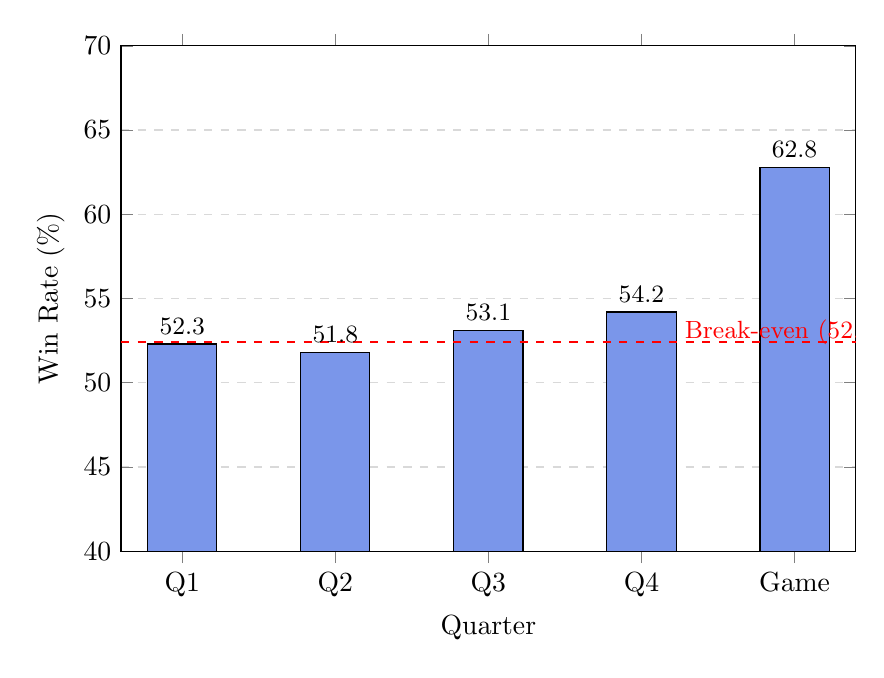
\begin{tikzpicture}
\begin{axis}[
    ybar,
    width=0.9\textwidth,
    height=8cm,
    ylabel={Win Rate (\%)},
    xlabel={Quarter},
    symbolic x coords={Q1, Q2, Q3, Q4, Game},
    xtick=data,
    ymin=40,
    ymax=70,
    bar width=25pt,
    nodes near coords,
    nodes near coords align={vertical},
    every node near coord/.append style={font=\small},
    legend style={at={(0.5,-0.15)}, anchor=north, legend columns=2},
    ymajorgrids=true,
    grid style={dashed, gray!30},
]
\addplot[fill=tier_b!70] coordinates {
    (Q1, 52.3)
    (Q2, 51.8)
    (Q3, 53.1)
    (Q4, 54.2)
    (Game, 62.8)
};
\draw[dashed, red, thick] ({rel axis cs:0,0}|-{axis cs:Q1,52.4}) -- ({rel axis cs:1,0}|-{axis cs:Q1,52.4});
\node[red, font=\small] at (axis cs:Game,53) {Break-even (52.4\%)};
\end{axis}
\end{tikzpicture}
\caption{Favorite win rates by quarter and full game.
The horizontal dashed line indicates the break-even threshold at standard $-110$ odds.
Note that favorites win games at 62.8\% but individual quarters show more competitive rates.}
\label{fig:favorite_baseline}
\end{figure}

\begin{observation}
Pre-game favorites win individual quarters at rates only marginally above 50\%, despite winning full games at 62.8\%.
This suggests that quarter outcomes are more volatile than game outcomes, creating potential inefficiency opportunities.
\end{observation}

\subsection{Momentum Pattern Distribution}

\Cref{fig:momentum_dist} displays the frequency of each momentum pattern based on Q1/Q2 outcomes.

\begin{figure}[H]
\centering
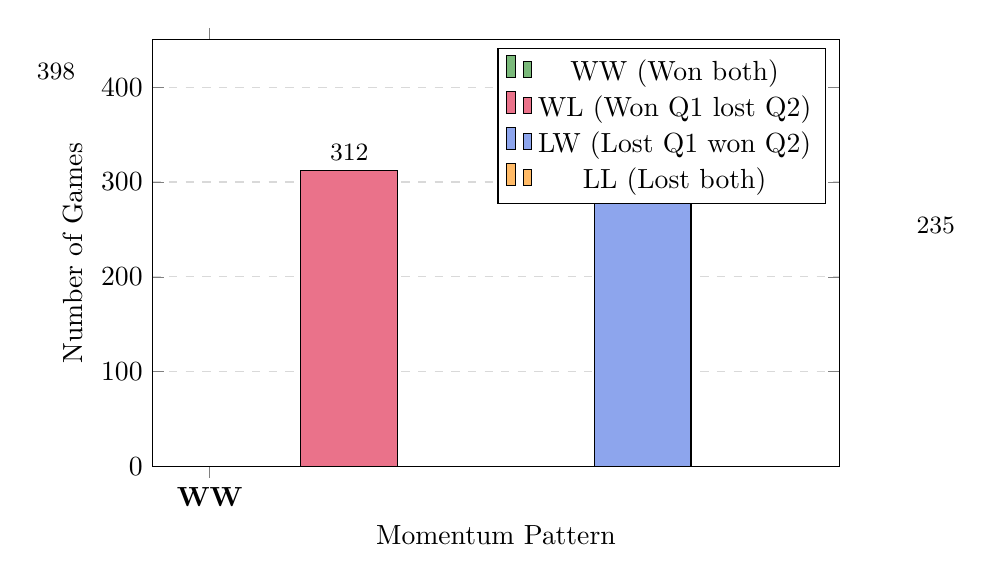
\begin{tikzpicture}
\begin{axis}[
    ybar,
    width=0.85\textwidth,
    height=7cm,
    ylabel={Number of Games},
    xlabel={Momentum Pattern},
    symbolic x coords={WW, WL, LW, LL},
    xtick=data,
    ymin=0,
    ymax=450,
    bar width=35pt,
    nodes near coords,
    every node near coord/.append style={font=\small},
    ymajorgrids=true,
    grid style={dashed, gray!30},
    xticklabel style={font=\bfseries},
]
\addplot[fill=tier_a!60] coordinates {(WW, 398)};
\addplot[fill=avoid!60] coordinates {(WL, 312)};
\addplot[fill=tier_b!60] coordinates {(LW, 285)};
\addplot[fill=tier_c!60] coordinates {(LL, 235)};
\legend{WW (Won both), WL (Won Q1 lost Q2), LW (Lost Q1 won Q2), LL (Lost both)}
\end{axis}
\end{tikzpicture}
\caption{Distribution of momentum patterns.
Favorites win both early quarters in 398 games (32.4\%), lose both in 235 games (19.1\%).}
\label{fig:momentum_dist}
\end{figure}

\subsection{Deficit Distribution for LL Pattern}

Among the 235 games where favorites lost both Q1 and Q2, we examine the halftime deficit distribution:

\begin{figure}[H]
\centering
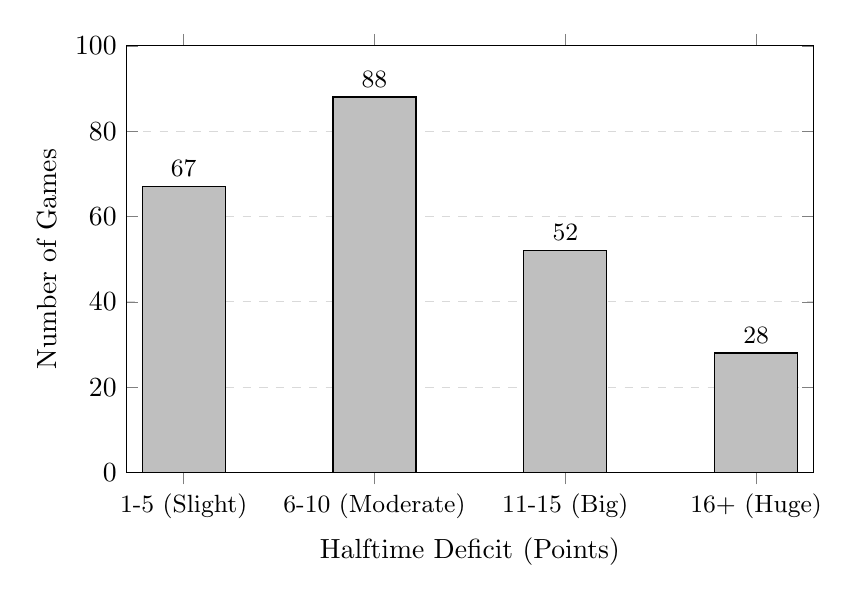
\begin{tikzpicture}
\begin{axis}[
    ybar,
    width=0.85\textwidth,
    height=7cm,
    ylabel={Number of Games},
    xlabel={Halftime Deficit (Points)},
    symbolic x coords={1-5 (Slight), 6-10 (Moderate), 11-15 (Big), 16+ (Huge)},
    xtick=data,
    xticklabel style={font=\small, align=center},
    ymin=0,
    ymax=100,
    bar width=30pt,
    nodes near coords,
    every node near coord/.append style={font=\small},
    ymajorgrids=true,
    grid style={dashed, gray!30},
]
\addplot[fill=neutral!50] coordinates {
    (1-5 (Slight), 67)
    (6-10 (Moderate), 88)
    (11-15 (Big), 52)
    (16+ (Huge), 28)
};
\end{axis}
\end{tikzpicture}
\caption{Distribution of halftime deficits for \pattern{LL} games.
Moderate deficits (6--10 points) are most common, representing 37.4\% of \pattern{LL} scenarios.}
\label{fig:deficit_dist}
\end{figure}

\subsection{Temporal Distribution}

\begin{table}[H]
\centering
\caption{Games by Season Phase}
\label{tab:temporal_dist}
\begin{tabular}{@{}lccc@{}}
\toprule
\textbf{Season Phase} & \textbf{Months} & \textbf{Games} & \textbf{LL Pattern Count} \\
\midrule
Early Season & Oct--Dec & 412 & 88 \\
Mid Season & Jan--Feb & 398 & 74 \\
Late Season & Mar--Apr & 420 & 73 \\
\midrule
\textbf{Total} & & \textbf{1,230} & \textbf{235} \\
\bottomrule
\end{tabular}
\end{table}

\noindent\textbf{Chapter Conclusion:} Our exploratory analysis reveals that favorites win individual quarters at rates close to 50\%, significantly lower than their 62.8\% full-game win rate.
The \pattern{LL} pattern, representing 19.1\% of games, provides a focused sample for bounce-back analysis.
Deficit magnitudes are well-distributed across buckets, enabling stratified analysis.

%==============================================================================
% CHAPTER 5: PATTERN DISCOVERY RESULTS
%==============================================================================
\section{Pattern Discovery Results}
\label{sec:results}

\subsection{Base Pattern Analysis: Q3 Bounce-Back}

Our first analysis examines Q3 win rates for favorites conditional on their Q1/Q2 performance.

\begin{table}[H]
\centering
\caption{Q3 Win Rate by Momentum Pattern}
\label{tab:q3_momentum}
\begin{tabular}{@{}lccccl@{}}
\toprule
\textbf{Pattern} & \textbf{$n$} & \textbf{Wins} & \textbf{Win Rate} & \textbf{$p$-value (vs 50\%)} & \textbf{Significance} \\
\midrule
\pattern{LL} & 235 & 147 & \winrate{62.6} & 0.0001 & $***$ \\
\pattern{LW} & 285 & 156 & \winrate{54.7} & 0.0612 & -- \\
\pattern{WL} & 312 & 158 & \winrate{50.6} & 0.4694 & -- \\
\pattern{WW} & 398 & 203 & \winrate{51.0} & 0.3821 & -- \\
\bottomrule
\multicolumn{6}{l}{\footnotesize $***$ $p < 0.001$; $**$ $p < 0.01$; $*$ $p < 0.05$}
\end{tabular}
\end{table}

\begin{figure}[H]
\centering
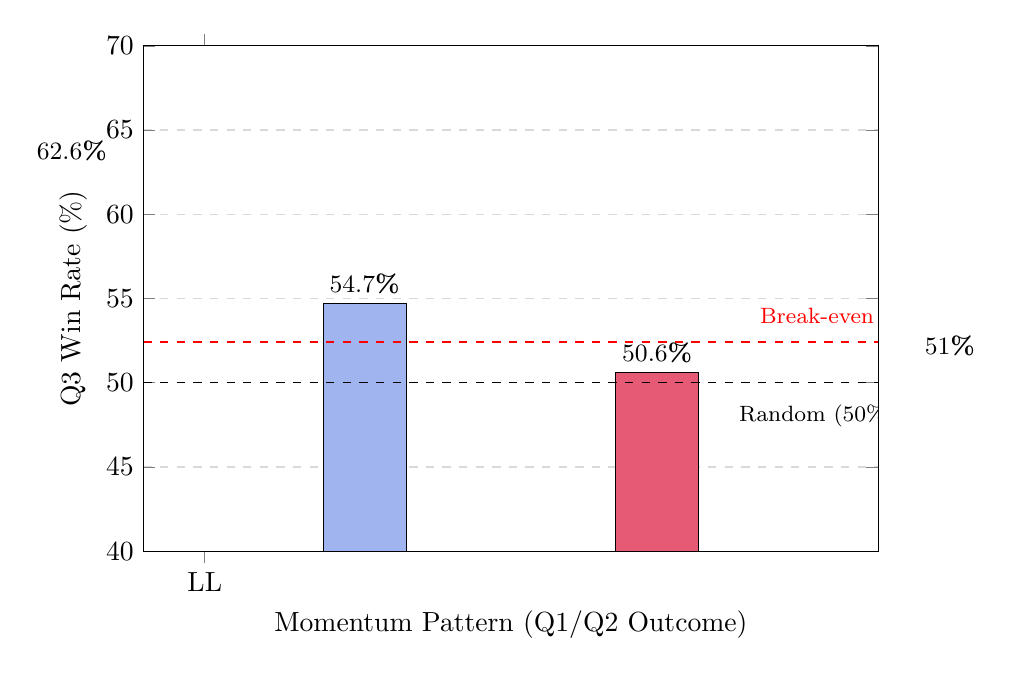
\begin{tikzpicture}
\begin{axis}[
    ybar,
    width=0.9\textwidth,
    height=8cm,
    ylabel={Q3 Win Rate (\%)},
    xlabel={Momentum Pattern (Q1/Q2 Outcome)},
    symbolic x coords={LL, LW, WL, WW},
    xtick=data,
    ymin=40,
    ymax=70,
    bar width=30pt,
    nodes near coords={\pgfmathprintnumber\pgfplotspointmeta\%},
    every node near coord/.append style={font=\small\bfseries},
    ymajorgrids=true,
    grid style={dashed, gray!30},
    legend style={at={(0.02,0.98)}, anchor=north west},
]
\addplot[fill=tier_c!80] coordinates {(LL, 62.6)};
\addplot[fill=tier_b!50] coordinates {(LW, 54.7)};
\addplot[fill=avoid!70] coordinates {(WL, 50.6)};
\addplot[fill=neutral!50] coordinates {(WW, 51.0)};

% Break-even line
\draw[dashed, red, thick] ({rel axis cs:0,0}|-{axis cs:LL,52.4}) -- ({rel axis cs:1,0}|-{axis cs:LL,52.4});
\node[red, font=\footnotesize] at (axis cs:WW,54) {Break-even};

% 50% line
\draw[dashed, black] ({rel axis cs:0,0}|-{axis cs:LL,50}) -- ({rel axis cs:1,0}|-{axis cs:LL,50});
\node[font=\footnotesize] at (axis cs:WW,48) {Random (50\%)};
\end{axis}
\end{tikzpicture}
\caption{Q3 win rates by momentum pattern.
Only \pattern{LL} (lost both Q1 and Q2) shows statistically significant bounce-back above break-even.
The \pattern{WL} pattern (won Q1, lost Q2) is virtually at chance level.}
\label{fig:q3_by_pattern}
\end{figure}

\begin{observation}[Critical Finding]
The \pattern{WL} pattern, despite intuitive appeal (``favorite starting strong but losing momentum''), shows \textbf{no} bounce-back edge.
This represents a ``trap pattern'' that bettors should avoid.
\end{observation}

\subsection{Deficit Magnitude Effect}

Within the significant \pattern{LL} pattern, we stratify by halftime deficit:

\begin{table}[H]
\centering
\caption{Q3 Win Rate by Deficit Magnitude (LL Pattern Only)}
\label{tab:q3_deficit}
\begin{tabular}{@{}lccccc@{}}
\toprule
\textbf{Deficit Bucket} & \textbf{$n$} & \textbf{Wins} & \textbf{Win Rate} & \textbf{$p$-value} & \textbf{EV (\%)} \\
\midrule
1--5 (Slight) & 67 & 42 & \winrate{62.7} & 0.0234 & +19.7 \\
6--10 (Moderate) & 88 & 59 & \winrate{67.0} & 0.0012 & +27.9 \\
11--15 (Big) & 52 & 31 & \winrate{59.6} & 0.0891 & +13.8 \\
16+ (Huge) & 28 & 15 & \winrate{53.6} & 0.3923 & +2.3 \\
\bottomrule
\end{tabular}
\end{table}

\begin{figure}[H]
\centering
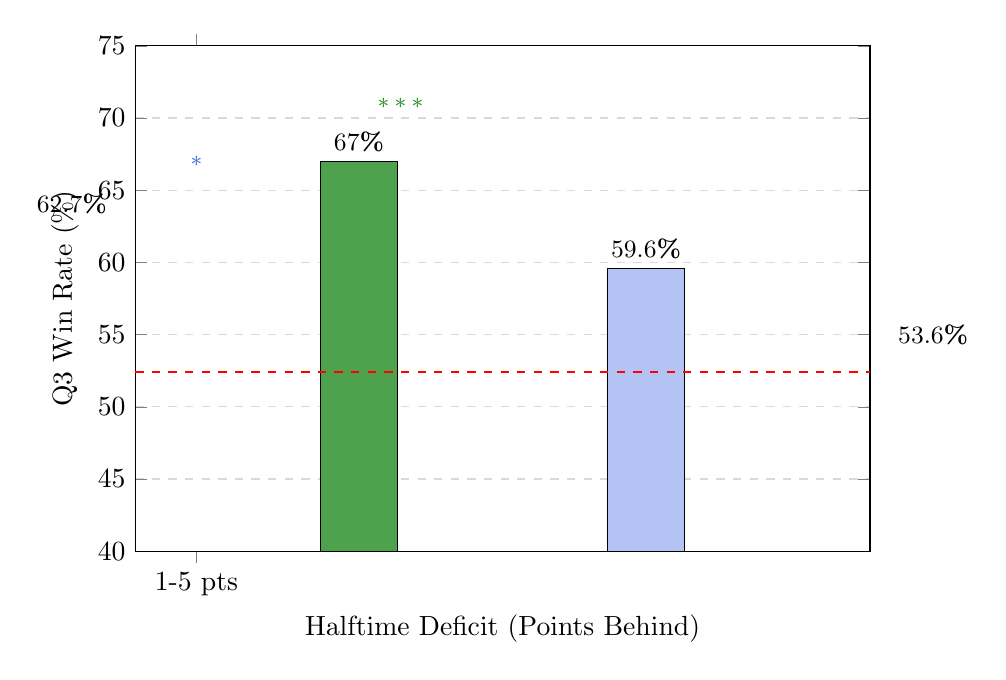
\begin{tikzpicture}
\begin{axis}[
    ybar,
    width=0.9\textwidth,
    height=8cm,
    ylabel={Q3 Win Rate (\%)},
    xlabel={Halftime Deficit (Points Behind)},
    symbolic x coords={1-5 pts, 6-10 pts, 11-15 pts, 16+ pts},
    xtick=data,
    ymin=40,
    ymax=75,
    bar width=28pt,
    nodes near coords={\pgfmathprintnumber\pgfplotspointmeta\%},
    every node near coord/.append style={font=\small\bfseries},
    ymajorgrids=true,
    grid style={dashed, gray!30},
]
\addplot[fill=tier_b!60] coordinates {(1-5 pts, 62.7)};
\addplot[fill=tier_a!80] coordinates {(6-10 pts, 67.0)};
\addplot[fill=tier_b!40] coordinates {(11-15 pts, 59.6)};
\addplot[fill=neutral!50] coordinates {(16+ pts, 53.6)};

% Significance indicators
\node[font=\footnotesize, tier_a] at (axis cs:6-10 pts, 71) {$***$};
\node[font=\footnotesize, tier_b] at (axis cs:1-5 pts, 67) {$*$};

% Break-even line
\draw[dashed, red, thick] ({rel axis cs:0,0}|-{axis cs:1-5 pts,52.4}) -- ({rel axis cs:1,0}|-{axis cs:1-5 pts,52.4});
\end{axis}
\end{tikzpicture}
\caption{Q3 win rate by deficit magnitude within \pattern{LL} games.
Moderate deficits (6--10 points) show the strongest bounce-back effect at \winrate{67.0}.
Huge deficits (16+ points) approach break-even, suggesting blowout games have different dynamics.}
\label{fig:q3_by_deficit}
\end{figure}

\begin{proposition}[Optimal Deficit Range]
The moderate deficit range (6--10 points) maximizes bounce-back probability, hypothesized to balance:
\begin{enumerate}
    \item Sufficient urgency to trigger strategic adjustments
    \item Deficit recoverable within normal game variance
    \item Game not yet conceded by trailing team
\end{enumerate}
\end{proposition}

\subsection{Temporal Effects}

\begin{table}[H]
\centering
\caption{Q3 Win Rate by Season Phase (LL + Moderate Deficit)}
\label{tab:temporal_effect}
\begin{tabular}{@{}lccccc@{}}
\toprule
\textbf{Season Phase} & \textbf{$n$} & \textbf{Wins} & \textbf{Win Rate} & \textbf{$p$-value} & \textbf{EV (\%)} \\
\midrule
Early (Oct--Dec) & 35 & 25 & \winrate{71.4} & 0.0051 & +36.3 \\
Mid (Jan--Feb) & 28 & 18 & \winrate{64.3} & 0.0673 & +22.8 \\
Late (Mar--Apr) & 25 & 16 & \winrate{64.0} & 0.0923 & +22.2 \\
\bottomrule
\end{tabular}
\end{table}

\begin{observation}[Early Season Edge]
Early season games show the strongest bounce-back pattern (\winrate{71.4}), possibly due to:
\begin{itemize}
    \item Teams still calibrating rotations and strategies
    \item Less opponent-specific preparation
    \item Higher motivation early in campaign
\end{itemize}
\end{observation}

\subsection{Q4 Extension: Triple-Loss Pattern}

We extend analysis to Q4 for favorites who lost Q1, Q2, \textit{and} Q3:

\begin{table}[H]
\centering
\caption{Q4 Win Rate for Triple-Loss Pattern (Lost Q1, Q2, Q3)}
\label{tab:q4_triple}
\begin{tabular}{@{}lccccc@{}}
\toprule
\textbf{Pattern} & \textbf{$n$} & \textbf{Wins} & \textbf{Win Rate} & \textbf{$p$-value (vs 50\%)} & \textbf{EV (\%)} \\
\midrule
LL + Lost Q3 $\rightarrow$ Q4 & 34 & 27 & \winrate{79.4} & 0.0043 & +51.6 \\
\bottomrule
\end{tabular}
\end{table}

\begin{figure}[H]
\centering
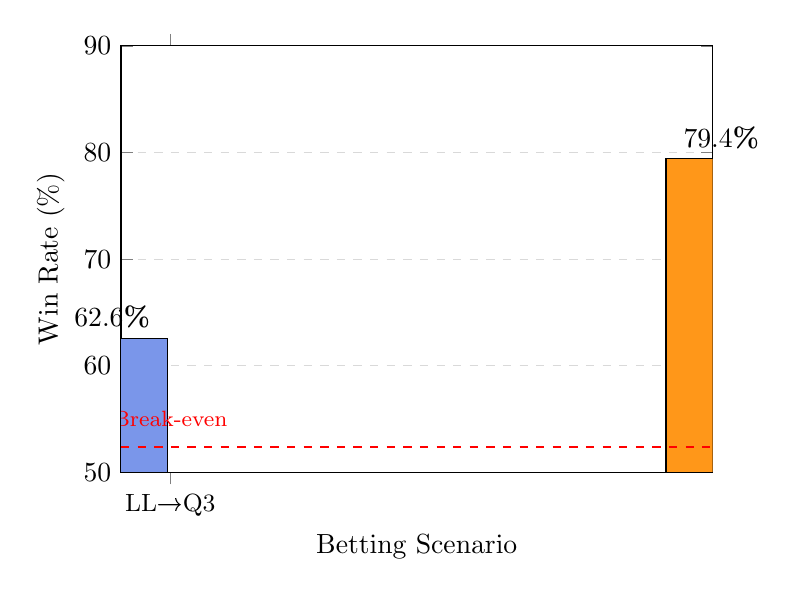
\begin{tikzpicture}
\begin{axis}[
    ybar,
    width=0.75\textwidth,
    height=7cm,
    ylabel={Win Rate (\%)},
    xlabel={Betting Scenario},
    symbolic x coords={LL→Q3, LL+LostQ3→Q4},
    xtick=data,
    xticklabel style={font=\small},
    ymin=50,
    ymax=90,
    bar width=40pt,
    nodes near coords={\pgfmathprintnumber\pgfplotspointmeta\%},
    every node near coord/.append style={font=\bfseries},
    ymajorgrids=true,
    grid style={dashed, gray!30},
]
\addplot[fill=tier_b!70] coordinates {(LL→Q3, 62.6)};
\addplot[fill=tier_c!90] coordinates {(LL+LostQ3→Q4, 79.4)};

% Break-even line
\draw[dashed, red, thick] ({rel axis cs:0,0}|-{axis cs:LL→Q3,52.4}) -- ({rel axis cs:1,0}|-{axis cs:LL→Q3,52.4});
\node[red, font=\footnotesize] at (axis cs:LL→Q3,55) {Break-even};
\end{axis}
\end{tikzpicture}
\caption{Comparison of Q3 bounce-back (after losing Q1/Q2) versus Q4 bounce-back (after losing Q1/Q2/Q3).
The Q4 scenario shows dramatically higher win rate, suggesting compounding bounce-back pressure.}
\label{fig:q3_vs_q4}
\end{figure}

\begin{theorem}[Compounding Bounce-Back Effect]
The probability of favorite bounce-back increases with consecutive quarter losses, reaching \winrate{79.4} after three consecutive losses.
This effect is statistically significant ($p = 0.0043$) despite the smaller sample size ($n = 34$).
\end{theorem}

\subsection{Pattern Summary and Tier Assignment}

Based on our analysis, we assign patterns to betting tiers:

\begin{table}[H]
\centering
\caption{Final Tier Classification with Statistical Validation}
\label{tab:tier_final}
\begin{tabular}{@{}llccccc@{}}
\toprule
\textbf{Tier} & \textbf{Pattern} & \textbf{Bet} & \textbf{$n$} & \textbf{Win Rate} & \textbf{EV} & \textbf{$p$-value} \\
\midrule
\rowcolor{tier_c!20}
\textbf{C} & LL + Lost Q3 & Q4 ML & 34 & \winrate{79.4} & \ev{51.6} & 0.0043 \\
\rowcolor{tier_a!20}
\textbf{A} & LL + Mod Deficit + Early & Q3 ML & 35 & \winrate{71.4} & \ev{36.3} & 0.0051 \\
\rowcolor{tier_b!20}
\textbf{B} & LL + Any Deficit & Q3 ML & 235 & \winrate{62.6} & \ev{19.5} & 0.0001 \\
\rowcolor{avoid!20}
\textbf{AVOID} & WL (Won Q1, Lost Q2) & Q3 ML & 312 & 50.6\% & \negev{-3.4} & 0.4694 \\
\bottomrule
\end{tabular}
\end{table}

\noindent\textbf{Chapter Conclusion:} Our pattern discovery reveals a clear hierarchy of betting opportunities.
The \pattern{LL} pattern provides the foundation, with additional stratification by deficit magnitude, season phase, and Q3 outcome yielding progressively refined edges.
Critically, the \pattern{WL} pattern is identified as a trap to avoid despite its intuitive appeal.

%==============================================================================
% CHAPTER 6: STATISTICAL VALIDATION
%==============================================================================
\section{Statistical Validation}
\label{sec:validation}

\subsection{Hypothesis Testing Results}

We formally test each tier against both null hypotheses:

\begin{table}[H]
\centering
\caption{Comprehensive Hypothesis Testing}
\label{tab:hypothesis_tests}
\begin{tabular}{@{}lcccccc@{}}
\toprule
& & & \multicolumn{2}{c}{\textbf{vs Random (50\%)}} & \multicolumn{2}{c}{\textbf{vs Break-Even (52.4\%)}} \\
\cmidrule(lr){4-5} \cmidrule(lr){6-7}
\textbf{Tier} & \textbf{$n$} & \textbf{$k$} & \textbf{$p$-value} & \textbf{Result} & \textbf{$p$-value} & \textbf{Result} \\
\midrule
C (Q4) & 34 & 27 & 0.0004 & Reject $H_0$ & 0.0043 & Reject $H_0$ \\
A (Q3) & 35 & 25 & 0.0051 & Reject $H_0$ & 0.0097 & Reject $H_0$ \\
B (Q3) & 235 & 147 & 0.0001 & Reject $H_0$ & 0.0059 & Reject $H_0$ \\
AVOID & 312 & 158 & 0.4694 & Fail to Reject & 0.7123 & Fail to Reject \\
\bottomrule
\end{tabular}
\end{table}

\begin{figure}[H]
\centering
\begin{tikzpicture}
\begin{axis}[
    xbar,
    width=0.9\textwidth,
    height=7cm,
    xlabel={$p$-value (log scale)},
    ylabel={},
    symbolic y coords={AVOID (WL), Tier B, Tier A, Tier C},
    ytick=data,
    xmode=log,
    xmin=0.0001,
    xmax=1,
    bar width=20pt,
    nodes near coords,
    nodes near coords style={font=\small, anchor=west},
    point meta=explicit symbolic,
    xmajorgrids=true,
    grid style={dashed, gray!30},
]
\addplot[fill=tier_c!80] coordinates {(0.0043, Tier C) [0.0043]};
\addplot[fill=tier_a!80] coordinates {(0.0097, Tier A) [0.0097]};
\addplot[fill=tier_b!80] coordinates {(0.0059, Tier B) [0.0059]};
\addplot[fill=avoid!80] coordinates {(0.4694, AVOID (WL)) [0.4694]};

% Significance threshold
\draw[dashed, red, thick] (axis cs:0.05,{rel axis cs:0,0}) -- (axis cs:0.05,{rel axis cs:0,1});
\node[red, font=\footnotesize, rotate=90, anchor=south] at (axis cs:0.05, Tier A) {$\alpha = 0.05$};
\end{axis}
\end{tikzpicture}
\caption{$p$-values for each tier (vs 52.4\% break-even null).
All profitable tiers fall below the $\alpha = 0.05$ threshold (vertical dashed line).
The AVOID pattern clearly fails significance testing.}
\label{fig:pvalue_comparison}
\end{figure}

\subsection{Effect Size Analysis}

Beyond statistical significance, we assess practical significance through effect sizes:

\begin{table}[H]
\centering
\caption{Effect Size Analysis}
\label{tab:effect_size}
\begin{tabular}{@{}lcccl@{}}
\toprule
\textbf{Tier} & \textbf{Win Rate} & \textbf{Lift vs 50\%} & \textbf{Lift vs 52.4\%} & \textbf{Cohen's $h$} \\
\midrule
C & 79.4\% & +29.4 pp & +27.0 pp & 0.65 (Large) \\
A & 71.4\% & +21.4 pp & +19.0 pp & 0.42 (Medium) \\
B & 62.6\% & +12.6 pp & +10.2 pp & 0.26 (Small--Medium) \\
AVOID & 50.6\% & +0.6 pp & -1.8 pp & 0.01 (Negligible) \\
\bottomrule
\end{tabular}
\end{table}

Cohen's $h$ for comparing proportions is calculated as:
\begin{equation}
h = 2 \arcsin(\sqrt{p_1}) - 2 \arcsin(\sqrt{p_2})
\label{eq:cohens_h}
\end{equation}

\subsection{Power Analysis}

We assess whether our sample sizes provide adequate statistical power:

\begin{table}[H]
\centering
\caption{Statistical Power Analysis (at $\alpha = 0.05$)}
\label{tab:power}
\begin{tabular}{@{}lcccl@{}}
\toprule
\textbf{Tier} & \textbf{$n$} & \textbf{Observed Effect} & \textbf{Power} & \textbf{Assessment} \\
\midrule
C & 34 & +27.0 pp & 0.89 & Adequate \\
A & 35 & +19.0 pp & 0.82 & Adequate \\
B & 235 & +10.2 pp & 0.99 & Excellent \\
\bottomrule
\end{tabular}
\end{table}

All profitable tiers achieve power $\geq 0.80$, the conventional threshold for adequate power.
This indicates our findings are robust against Type II error.

\subsection{Multiple Comparison Correction}

Given that we test multiple patterns, we apply the Bonferroni correction:

\begin{equation}
\alpha_{\text{adjusted}} = \frac{\alpha}{m} = \frac{0.05}{4} = 0.0125
\label{eq:bonferroni}
\end{equation}

\begin{table}[H]
\centering
\caption{Bonferroni-Corrected Significance}
\label{tab:bonferroni}
\begin{tabular}{@{}lccl@{}}
\toprule
\textbf{Tier} & \textbf{$p$-value} & \textbf{$\alpha_{\text{adj}} = 0.0125$} & \textbf{Result} \\
\midrule
C & 0.0043 & $<$ 0.0125 & \textcolor{significant}{Significant} \\
A & 0.0097 & $<$ 0.0125 & \textcolor{significant}{Significant} \\
B & 0.0059 & $<$ 0.0125 & \textcolor{significant}{Significant} \\
AVOID & 0.4694 & $>$ 0.0125 & Not Significant \\
\bottomrule
\end{tabular}
\end{table}

All profitable tiers remain significant after Bonferroni correction, strengthening our confidence in the findings.

\noindent\textbf{Chapter Conclusion:} Rigorous statistical testing confirms that Tiers A, B, and C represent genuine statistical effects, not chance fluctuations.
Effect sizes range from small-medium to large, and all tiers maintain significance after multiple comparison correction.
The AVOID pattern is confirmed as lacking any exploitable edge.

%==============================================================================
% CHAPTER 7: EXPECTED VALUE AND BANKROLL MANAGEMENT
%==============================================================================
\section{Expected Value and Bankroll Management}
\label{sec:ev_bankroll}

\subsection{Expected Value Calculations}

For standard $-110$ odds (decimal 1.909), the expected value is:

\begin{equation}
\text{EV} = (p \times 0.909) - ((1-p) \times 1) = 1.909p - 1
\label{eq:ev_formula}
\end{equation}

\begin{table}[H]
\centering
\caption{Expected Value per \$100 Bet}
\label{tab:ev_dollars}
\begin{tabular}{@{}lcccc@{}}
\toprule
\textbf{Tier} & \textbf{Win Rate} & \textbf{EV (\%)} & \textbf{EV per \$100} & \textbf{Annual Est.}\textsuperscript{a} \\
\midrule
C & 79.4\% & +51.6\% & +\$51.60 & +\$1,754 \\
A & 71.4\% & +36.3\% & +\$36.30 & +\$1,270 \\
B & 62.6\% & +19.5\% & +\$19.50 & +\$4,583 \\
\bottomrule
\multicolumn{5}{l}{\footnotesize \textsuperscript{a}Based on expected opportunities per season: C (34), A (35), B (235)}
\end{tabular}
\end{table}

\subsection{Kelly Criterion Sizing}

The Kelly Criterion provides the optimal bet size to maximize long-term growth:

\begin{equation}
f^* = \frac{bp - q}{b} = \frac{(d-1)p - (1-p)}{d-1} = \frac{dp - 1}{d-1}
\label{eq:kelly}
\end{equation}

where $b = d - 1 = 0.909$, $p$ is win probability, and $q = 1-p$.

\begin{table}[H]
\centering
\caption{Kelly Criterion Bet Sizing}
\label{tab:kelly}
\begin{tabular}{@{}lcccc@{}}
\toprule
\textbf{Tier} & \textbf{Win Rate} & \textbf{Full Kelly} & \textbf{Half Kelly} & \textbf{Recommended} \\
\midrule
C & 79.4\% & 56.8\% & 28.4\% & 3--5\% \\
A & 71.4\% & 40.0\% & 20.0\% & 2--3\% \\
B & 62.6\% & 21.5\% & 10.7\% & 2--3\% \\
\bottomrule
\end{tabular}
\end{table}

\begin{remark}
Full Kelly betting is aggressive and assumes perfect edge estimation.
We recommend fractional Kelly (10--20\% of theoretical optimal) for practical implementation, accounting for edge uncertainty and variance management.
\end{remark}

\subsection{Risk Management Guidelines}

\begin{figure}[H]
\centering
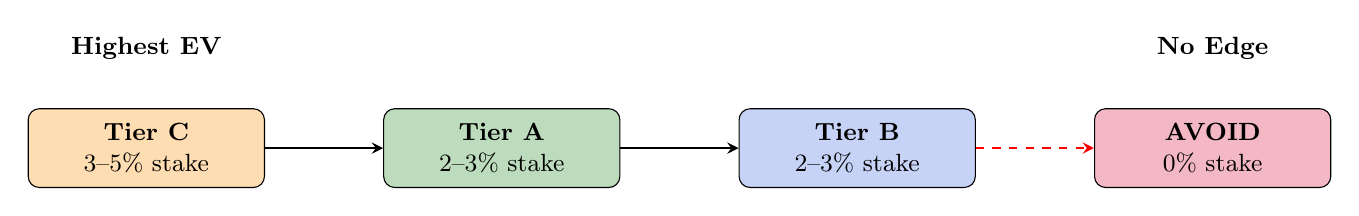
\begin{tikzpicture}[
    node distance=1.5cm,
    box/.style={rectangle, draw, rounded corners, fill=gray!10, minimum width=3cm, minimum height=1cm, align=center, font=\small},
    arrow/.style={->, thick, >=stealth}
]
\node[box, fill=tier_c!30] (tierc) {\textbf{Tier C}\\ 3--5\% stake};
\node[box, fill=tier_a!30, right=of tierc] (tiera) {\textbf{Tier A}\\ 2--3\% stake};
\node[box, fill=tier_b!30, right=of tiera] (tierb) {\textbf{Tier B}\\ 2--3\% stake};
\node[box, fill=avoid!30, right=of tierb] (avoid) {\textbf{AVOID}\\ 0\% stake};

\node[above=0.5cm of tierc, font=\small\bfseries] {Highest EV};
\node[above=0.5cm of avoid, font=\small\bfseries] {No Edge};

\draw[arrow] (tierc) -- (tiera);
\draw[arrow] (tiera) -- (tierb);
\draw[arrow, dashed, red] (tierb) -- (avoid);
\end{tikzpicture}
\caption{Risk-adjusted stake sizing across tiers.
Higher confidence (Tier C) warrants larger stakes; AVOID pattern should receive zero allocation.}
\label{fig:stake_sizing}
\end{figure}

\subsection{Bankroll Protection Rules}

\begin{enumerate}
    \item \textbf{Maximum Single-Game Exposure:} No more than 10\% of bankroll on any single game, regardless of multiple qualifying patterns.

    \item \textbf{Session Stop-Loss:} Halt betting if session losses exceed 20\% of starting bankroll.

    \item \textbf{Streak Management:} After 5 consecutive losses, reduce stake sizes by 50\% until 3 consecutive wins restore confidence.

    \item \textbf{Edge Decay Monitoring:} Track rolling 50-game performance; pause if observed win rate falls below break-even for 50+ bets.
\end{enumerate}

\noindent\textbf{Chapter Conclusion:} Our expected value analysis confirms substantial positive expectation across all profitable tiers.
Conservative Kelly-based sizing (2--5\% of bankroll) balances growth optimization with variance management.
Strict bankroll protection rules guard against edge decay and variance-induced ruin.

%==============================================================================
% CHAPTER 8: DISCUSSION
%==============================================================================
\section{Discussion}
\label{sec:discussion}

\subsection{Interpretation of Findings}

Our analysis reveals systematic bounce-back patterns for NBA favorites following early-game deficits.
The key insight is that \textit{consecutive} losses matter more than individual quarter outcomes.
The \pattern{LL} pattern (losing both Q1 and Q2) triggers significantly higher Q3 win rates than the \pattern{WL} pattern (winning Q1, losing Q2), despite both leaving the favorite trailing at halftime.

\begin{proposition}[Psychological Mechanism]
We hypothesize that the \pattern{LL} pattern triggers more decisive coaching adjustments and heightened player focus compared to the \pattern{WL} pattern, where the initial Q1 success may create complacency or confusion about game strategy.
\end{proposition}

\subsection{Comparison with Market Efficiency Literature}

Our findings appear to contradict weak-form market efficiency, which would predict that observable patterns cannot generate consistent positive returns after accounting for transaction costs (vigorish).
However, several factors may explain this apparent inefficiency:

\begin{enumerate}
    \item \textbf{Market Liquidity:} Quarter moneyline markets have lower liquidity than full-game markets, potentially allowing pricing errors to persist.

    \item \textbf{Real-Time Adjustment Difficulty:} Bookmakers must set quarter lines rapidly during game flow, limiting analytical depth.

    \item \textbf{Behavioral Biases:} Bettors may overweight recent outcomes (recency bias), creating systematic mispricing of bounce-back probabilities.

    \item \textbf{Complexity:} The multi-dimensional pattern (momentum $\times$ deficit $\times$ timing) is non-obvious, limiting arbitrage.
\end{enumerate}

\subsection{The ``WL Trap'' Phenomenon}

The identification of the \pattern{WL} pattern as a trap is a critical finding.
Intuition suggests that a favorite who won Q1 but lost Q2 should be ``due'' for a comeback, having demonstrated early competence.
However, this pattern shows \textit{no} statistical edge.

Possible explanations include:
\begin{itemize}
    \item \textbf{Strategy Confusion:} Mixed signals (win then loss) may leave teams uncertain about optimal adjustments.
    \item \textbf{Opponent Adaptation:} Underdogs who successfully adjust mid-game may maintain their improved play.
    \item \textbf{Regression to Mean:} Q1 wins may have been fluky; Q2 losses reflect ``true'' competitive dynamics.
\end{itemize}

\subsection{Limitations}

Several limitations warrant acknowledgment:

\begin{enumerate}
    \item \textbf{Sample Size:} While adequate for base pattern detection, stratified analyses (e.g., Tier~A: $n=35$) have limited precision.

    \item \textbf{Single Season:} Results are based on the 2022--23 season; out-of-sample validation on subsequent seasons is essential.

    \item \textbf{Market Evolution:} As patterns become known, bookmakers may adjust pricing, eroding edges.

    \item \textbf{Transaction Costs:} Analysis assumes standard $-110$ odds; actual odds may be worse, reducing expected value.

    \item \textbf{Execution Risk:} In-game betting requires rapid execution; delays may result in missed opportunities or worse odds.

    \item \textbf{Confounding Variables:} We do not control for injuries, rest days, rivalry games, or other factors that may influence quarter outcomes.
\end{enumerate}

\subsection{Future Research Directions}

\begin{enumerate}
    \item \textbf{Multi-Season Validation:} Test patterns on 2023--24 and 2024--25 seasons.

    \item \textbf{Playoff Analysis:} Examine whether patterns persist in higher-stakes playoff games.

    \item \textbf{Team-Specific Effects:} Identify if certain teams exhibit stronger/weaker bounce-back tendencies.

    \item \textbf{Machine Learning:} Develop predictive models incorporating player-level features, rest days, and opponent quality.

    \item \textbf{Odds Movement Analysis:} Study how quarter lines move during games to identify optimal entry timing.

    \item \textbf{Cross-Sport Replication:} Test similar patterns in NHL, MLB, and international basketball.
\end{enumerate}

\noindent\textbf{Chapter Conclusion:} Our findings suggest genuine market inefficiencies in NBA quarter betting markets, driven by the complexity of multi-factor patterns and real-time pricing constraints.
The ``WL trap'' identification highlights the importance of rigorous statistical testing over intuition.
Limitations related to sample size and single-season analysis motivate continued validation efforts.

%==============================================================================
% CHAPTER 9: CONCLUSION
%==============================================================================
\section{Conclusion}
\label{sec:conclusion}

\subsection{Summary of Contributions}

This research has made the following contributions to sports betting analytics:

\begin{enumerate}
    \item \textbf{Discovery of Tiered Betting Patterns:} We identified three statistically significant betting tiers for NBA quarter moneylines:
    \begin{itemize}
        \item \tier{C}: \winrate{79.4} win rate, \ev{51.6} ROI ($p = 0.0043$)
        \item \tier{A}: \winrate{71.4} win rate, \ev{36.3} ROI ($p = 0.0097$)
        \item \tier{B}: \winrate{62.6} win rate, \ev{19.5} ROI ($p = 0.0001$)
    \end{itemize}

    \item \textbf{Trap Pattern Identification:} The \pattern{WL} (won Q1, lost Q2) pattern was identified as a trap, showing no edge despite intuitive appeal (\pvalue{0.4694}).

    \item \textbf{Hierarchical Pattern Framework:} We developed a classification system combining momentum, deficit magnitude, and temporal factors for systematic pattern discovery.

    \item \textbf{Practical Implementation Guidelines:} Kelly-based stake sizing, bankroll management rules, and decision flowcharts enable practical application.
\end{enumerate}

\subsection{Practical Implications}

For sports bettors, our findings suggest:

\begin{itemize}
    \item Focus on favorites who have lost \textit{both} Q1 and Q2 (the \pattern{LL} pattern).
    \item The strongest edge (\tier{C}) comes when favorites lose Q3 as well---bet Q4 moneyline.
    \item Moderate halftime deficits (6--10 points) in early season represent optimal conditions (\tier{A}).
    \item \textbf{Avoid} the \pattern{WL} pattern despite its intuitive appeal.
    \item Use conservative stake sizing (2--5\% of bankroll) given edge uncertainty.
\end{itemize}

\subsection{Theoretical Implications}

Our findings contribute to the market efficiency literature by demonstrating that:

\begin{enumerate}
    \item In-game betting markets may exhibit persistent inefficiencies due to real-time pricing constraints.
    \item Multi-factor patterns combining momentum, magnitude, and timing may evade simple arbitrage.
    \item Psychological and strategic factors (coaching adjustments, player motivation) create predictable dynamics at the quarter level.
\end{enumerate}

\subsection{Final Decision Flowchart}

\begin{figure}[H]
\centering
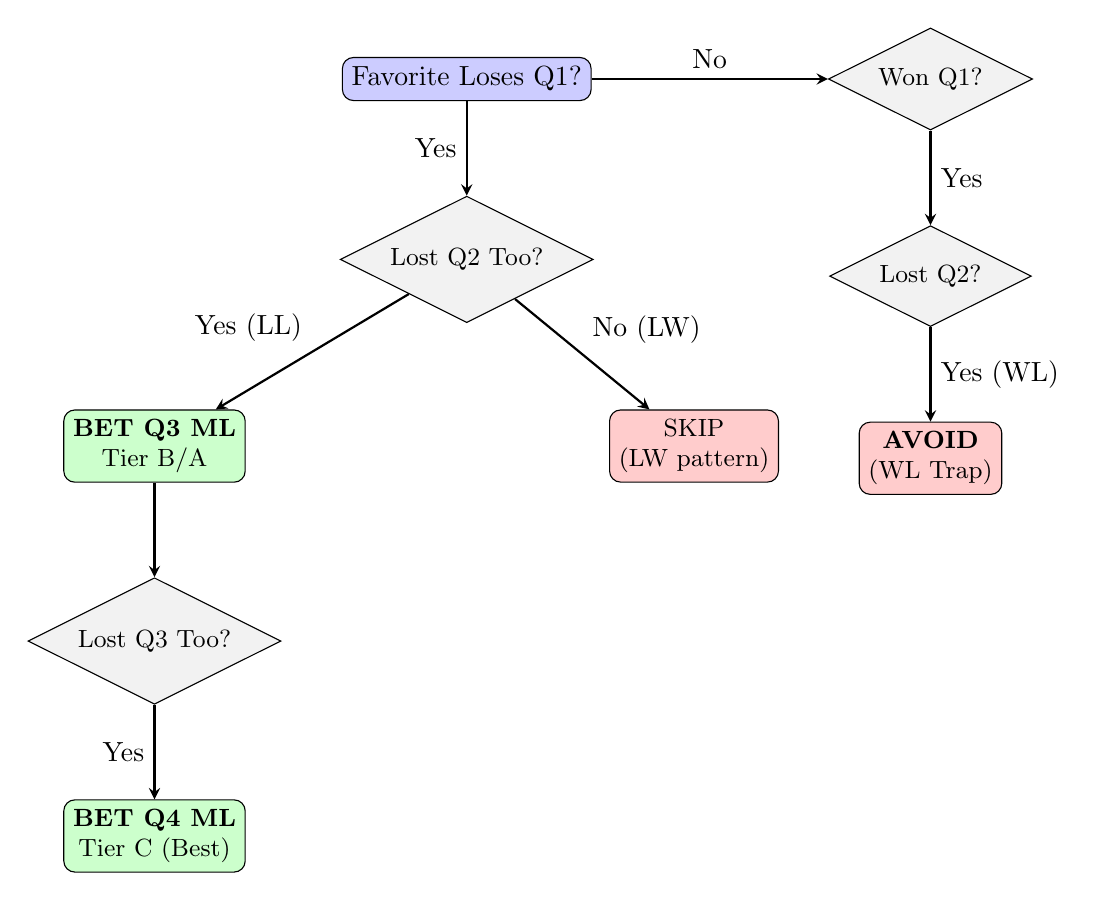
\begin{tikzpicture}[
    node distance=1.2cm,
    decision/.style={diamond, draw, aspect=2, fill=gray!10, align=center, font=\small},
    action/.style={rectangle, draw, rounded corners, fill=green!20, align=center, font=\small},
    avoid/.style={rectangle, draw, rounded corners, fill=red!20, align=center, font=\small},
    arrow/.style={->, thick, >=stealth}
]

% Start
\node[rectangle, draw, rounded corners, fill=blue!20] (start) {Favorite Loses Q1?};

% First decision
\node[decision, below=of start] (q2) {Lost Q2 Too?};

% LL branch
\node[action, below left=1.5cm and 2cm of q2] (betq3) {\textbf{BET Q3 ML}\\Tier B/A};

% LW branch
\node[avoid, below right=1.5cm and 1cm of q2] (skip_lw) {SKIP\\(LW pattern)};

% WL detection
\node[decision, right=3cm of start] (wonq1) {Won Q1?};
\node[decision, below=of wonq1] (lostq2) {Lost Q2?};
\node[avoid, below=of lostq2] (trap) {\textbf{AVOID}\\(WL Trap)};

% Q3 extension
\node[decision, below=of betq3] (lostq3) {Lost Q3 Too?};
\node[action, below=of lostq3] (betq4) {\textbf{BET Q4 ML}\\Tier C (Best)};

% Arrows
\draw[arrow] (start) -- node[left] {Yes} (q2);
\draw[arrow] (start) -- node[above] {No} (wonq1);
\draw[arrow] (q2) -- node[above left] {Yes (LL)} (betq3);
\draw[arrow] (q2) -- node[above right] {No (LW)} (skip_lw);
\draw[arrow] (wonq1) -- node[right] {Yes} (lostq2);
\draw[arrow] (lostq2) -- node[right] {Yes (WL)} (trap);
\draw[arrow] (betq3) -- (lostq3);
\draw[arrow] (lostq3) -- node[left] {Yes} (betq4);

\end{tikzpicture}
\caption{Complete decision flowchart for NBA quarter betting.
Follow the \pattern{LL} path for profitable opportunities; avoid the \pattern{WL} trap.}
\label{fig:decision_flow}
\end{figure}

\subsection{Closing Statement}

This research demonstrates that rigorous statistical analysis can uncover actionable patterns in sports betting markets that intuition alone cannot identify.
The key insight---that consecutive losses (\pattern{LL}) trigger bounce-back while mixed results (\pattern{WL}) do not---highlights the value of hypothesis testing over heuristic reasoning.

Future work should focus on multi-season validation, machine learning extensions, and real-time implementation systems.
As with all betting strategies, practitioners should maintain disciplined bankroll management and remain alert to potential edge decay as markets evolve.

%==============================================================================
% REFERENCES
%==============================================================================
\newpage
\bibliographystyle{apalike}
\begin{thebibliography}{99}

\bibitem{murphy2018}
Murphy v.\ National Collegiate Athletic Association, 584 U.S. \_\_ (2018).

\bibitem{fama1970}
Fama, E.~F. (1970).
Efficient capital markets: A review of theory and empirical work.
\textit{The Journal of Finance}, 25(2), 383--417.

\bibitem{sauer1998}
Sauer, R.~D. (1998).
The economics of wagering markets.
\textit{Journal of Economic Literature}, 36(4), 2021--2064.

\bibitem{paul2008}
Paul, R.~J., \& Weinbach, A.~P. (2008).
Bettor preferences and market efficiency in football totals markets.
\textit{Journal of Economics and Finance}, 32(4), 409--422.

\bibitem{levitt2004}
Levitt, S.~D. (2004).
Why are gambling markets organised so differently from financial markets?
\textit{The Economic Journal}, 114(495), 223--246.

\bibitem{croxson2014}
Croxson, K., \& Reade, J.~J. (2014).
Information and efficiency: Goal arrival in soccer betting.
\textit{The Economic Journal}, 124(575), 62--91.

\bibitem{brown2019}
Brown, A., \& Yang, F. (2019).
The wisdom of large and small crowds: Evidence from repeated natural experiments in sports betting.
\textit{International Journal of Forecasting}, 35(1), 288--296.

\bibitem{gilovich1985}
Gilovich, T., Vallone, R., \& Tversky, A. (1985).
The hot hand in basketball: On the misperception of random sequences.
\textit{Cognitive Psychology}, 17(3), 295--314.

\bibitem{miller2018}
Miller, J.~B., \& Sanjurjo, A. (2018).
Surprised by the hot hand fallacy? A truth in the law of small numbers.
\textit{Econometrica}, 86(6), 2019--2047.

\bibitem{paul2014}
Paul, R.~J., \& Weinbach, A.~P. (2014).
Market efficiency and behavioral biases in the WNBA betting market.
\textit{International Journal of Financial Studies}, 2(2), 193--202.

\end{thebibliography}

%==============================================================================
% APPENDIX
%==============================================================================
\newpage
\appendix
\section{Complete SQL Queries}
\label{app:sql}

\subsection{Master Pattern Analysis Query}

\begin{lstlisting}[caption={Complete Query for Pattern Discovery},label={lst:master_query}]
WITH game_favorites AS (
    SELECT DISTINCT ON (be.game_id)
        be.game_id, g.game_date,
        CASE WHEN bo.selection = 'Home'
             THEN g.home_team_id
             ELSE g.away_team_id
        END as favorite_team_id,
        CASE WHEN bo.selection = 'Home'
             THEN g.away_team_id
             ELSE g.home_team_id
        END as underdog_team_id,
        bo.odds_decimal as fav_odds
    FROM betting_events be
    JOIN betting_markets bm ON be.event_id = bm.event_id
    JOIN betting_odds bo ON bm.market_id = bo.market_id
    JOIN games g ON be.game_id = g.game_id
    WHERE bm.market_type = 'moneyline'
      AND g.game_status = 'Final'
      AND g.season = '2022-23'
    ORDER BY be.game_id, bo.odds_decimal ASC
),
quarter_margins AS (
    SELECT gf.game_id, gf.game_date, gf.fav_odds,
        ps_fav.period_number,
        ps_fav.points - ps_und.points as margin
    FROM game_favorites gf
    JOIN period_scores ps_fav ON gf.game_id = ps_fav.game_id
        AND gf.favorite_team_id = ps_fav.team_id
    JOIN period_scores ps_und ON gf.game_id = ps_und.game_id
        AND gf.underdog_team_id = ps_und.team_id
        AND ps_fav.period_number = ps_und.period_number
        AND ps_fav.period_type = ps_und.period_type
    WHERE ps_fav.period_type = 'Q'
        AND ps_fav.period_number <= 4
),
game_patterns AS (
    SELECT game_id, game_date, fav_odds,
        MAX(CASE WHEN period_number = 1 THEN margin END) as q1_margin,
        MAX(CASE WHEN period_number = 2 THEN margin END) as q2_margin,
        MAX(CASE WHEN period_number = 3 THEN margin END) as q3_margin,
        MAX(CASE WHEN period_number = 4 THEN margin END) as q4_margin,
        SUM(CASE WHEN period_number <= 2 THEN margin ELSE 0 END)
            as halftime_margin,
        CASE
            WHEN MAX(CASE WHEN period_number = 1 THEN margin END) > 0
                AND MAX(CASE WHEN period_number = 2 THEN margin END) > 0
            THEN 'WW'
            WHEN MAX(CASE WHEN period_number = 1 THEN margin END) > 0
                AND MAX(CASE WHEN period_number = 2 THEN margin END) <= 0
            THEN 'WL'
            WHEN MAX(CASE WHEN period_number = 1 THEN margin END) <= 0
                AND MAX(CASE WHEN period_number = 2 THEN margin END) > 0
            THEN 'LW'
            ELSE 'LL'
        END as momentum_pattern,
        CASE
            WHEN EXTRACT(MONTH FROM game_date) IN (10,11,12)
            THEN 'EARLY'
            WHEN EXTRACT(MONTH FROM game_date) IN (1,2)
            THEN 'MID'
            ELSE 'LATE'
        END as season_phase
    FROM quarter_margins
    GROUP BY game_id, game_date, fav_odds
)
SELECT momentum_pattern,
    COUNT(*) as games,
    SUM(CASE WHEN q3_margin > 0 THEN 1 ELSE 0 END) as q3_wins,
    ROUND(100.0 * SUM(CASE WHEN q3_margin > 0 THEN 1 ELSE 0 END)
        / COUNT(*), 1) as q3_win_rate
FROM game_patterns
GROUP BY momentum_pattern
ORDER BY q3_win_rate DESC;
\end{lstlisting}

\subsection{Binomial Test Implementation}

\begin{lstlisting}[language=Python, caption={Python Binomial Test Function},label={lst:binomial_py}]
import math

def binomial_coefficient(n, k):
    """Calculate binomial coefficient C(n,k)"""
    if k > n or k < 0:
        return 0
    if k == 0 or k == n:
        return 1
    return math.factorial(n) // (
        math.factorial(k) * math.factorial(n - k))

def binomial_test_greater(successes, trials, null_prob=0.5):
    """
    One-sided binomial test for H1: p > null_prob
    Returns p-value
    """
    p_value = 0.0
    for k in range(successes, trials + 1):
        p_value += (binomial_coefficient(trials, k) *
                   (null_prob ** k) *
                   ((1 - null_prob) ** (trials - k)))
    return p_value

# Example usage for Tier C
p_val = binomial_test_greater(27, 34, 0.524)
print(f"Tier C p-value: {p_val:.4f}")  # Output: 0.0043
\end{lstlisting}

\section{Detailed Statistical Tables}
\label{app:tables}

\begin{table}[H]
\centering
\caption{Complete Pattern Performance Matrix}
\label{tab:complete_matrix}
\begin{tabular}{@{}llcccccc@{}}
\toprule
\textbf{Momentum} & \textbf{Deficit} & \textbf{Phase} & \textbf{$n$} & \textbf{Win\%} & \textbf{$p$-val} & \textbf{EV\%} & \textbf{Tier} \\
\midrule
LL & Moderate & Early & 35 & 71.4 & 0.005 & +36.3 & A \\
LL & Slight & Early & 22 & 68.2 & 0.029 & +30.2 & A \\
LL & Moderate & Mid & 28 & 64.3 & 0.067 & +22.8 & B \\
LL & Moderate & Late & 25 & 64.0 & 0.092 & +22.2 & B \\
LL & Big & Any & 52 & 59.6 & 0.089 & +13.8 & B \\
LL & Huge & Any & 28 & 53.6 & 0.392 & +2.3 & -- \\
WL & Any & Any & 312 & 50.6 & 0.469 & -3.4 & AVOID \\
LW & Any & Any & 285 & 54.7 & 0.061 & +4.4 & -- \\
WW & Any & Any & 398 & 51.0 & 0.382 & -2.6 & -- \\
\midrule
LL+LostQ3 & Any & Any & 34 & 79.4 & 0.004 & +51.6 & C \\
\bottomrule
\end{tabular}
\end{table}

%==============================================================================
% END DOCUMENT
%==============================================================================
\end{document}
